\documentclass[]{article}
\usepackage{lmodern}
\usepackage{amssymb,amsmath}
\usepackage{ifxetex,ifluatex}
\usepackage{fixltx2e} % provides \textsubscript
\ifnum 0\ifxetex 1\fi\ifluatex 1\fi=0 % if pdftex
  \usepackage[T1]{fontenc}
  \usepackage[utf8]{inputenc}
\else % if luatex or xelatex
  \ifxetex
    \usepackage{mathspec}
  \else
    \usepackage{fontspec}
  \fi
  \defaultfontfeatures{Ligatures=TeX,Scale=MatchLowercase}
\fi
% use upquote if available, for straight quotes in verbatim environments
\IfFileExists{upquote.sty}{\usepackage{upquote}}{}
% use microtype if available
\IfFileExists{microtype.sty}{%
\usepackage{microtype}
\UseMicrotypeSet[protrusion]{basicmath} % disable protrusion for tt fonts
}{}
\usepackage[margin=1in]{geometry}
\usepackage{hyperref}
\hypersetup{unicode=true,
            pdftitle={Assignment 3},
            pdfauthor={Sri Seshadri},
            pdfborder={0 0 0},
            breaklinks=true}
\urlstyle{same}  % don't use monospace font for urls
\usepackage{graphicx,grffile}
\makeatletter
\def\maxwidth{\ifdim\Gin@nat@width>\linewidth\linewidth\else\Gin@nat@width\fi}
\def\maxheight{\ifdim\Gin@nat@height>\textheight\textheight\else\Gin@nat@height\fi}
\makeatother
% Scale images if necessary, so that they will not overflow the page
% margins by default, and it is still possible to overwrite the defaults
% using explicit options in \includegraphics[width, height, ...]{}
\setkeys{Gin}{width=\maxwidth,height=\maxheight,keepaspectratio}
\IfFileExists{parskip.sty}{%
\usepackage{parskip}
}{% else
\setlength{\parindent}{0pt}
\setlength{\parskip}{6pt plus 2pt minus 1pt}
}
\setlength{\emergencystretch}{3em}  % prevent overfull lines
\providecommand{\tightlist}{%
  \setlength{\itemsep}{0pt}\setlength{\parskip}{0pt}}
\setcounter{secnumdepth}{0}
% Redefines (sub)paragraphs to behave more like sections
\ifx\paragraph\undefined\else
\let\oldparagraph\paragraph
\renewcommand{\paragraph}[1]{\oldparagraph{#1}\mbox{}}
\fi
\ifx\subparagraph\undefined\else
\let\oldsubparagraph\subparagraph
\renewcommand{\subparagraph}[1]{\oldsubparagraph{#1}\mbox{}}
\fi

%%% Use protect on footnotes to avoid problems with footnotes in titles
\let\rmarkdownfootnote\footnote%
\def\footnote{\protect\rmarkdownfootnote}

%%% Change title format to be more compact
\usepackage{titling}

% Create subtitle command for use in maketitle
\newcommand{\subtitle}[1]{
  \posttitle{
    \begin{center}\large#1\end{center}
    }
}

\setlength{\droptitle}{-2em}
  \title{Assignment 3}
  \pretitle{\vspace{\droptitle}\centering\huge}
  \posttitle{\par}
  \author{Sri Seshadri}
  \preauthor{\centering\large\emph}
  \postauthor{\par}
  \predate{\centering\large\emph}
  \postdate{\par}
  \date{8/5/2018}

\usepackage{float}

\begin{document}
\maketitle

\section{Problem 1}\label{problem-1}

Here there are two scenarios that will be inspected using Integer Linear
Programming (ILP) to model total cost. Scenario 1 - plant in Baltimore,
Scenario 2 - plant in Seattle.

\subsection{Scenario 1}\label{scenario-1}

\subsubsection{Formulation:}\label{formulation}

The model is formulated as a network flow model as shown in the figure
below, where nodes 1 through 5 are Los Angeles, Baltimore, Atlanta,
Tulsa and New York respectively

\begin{center}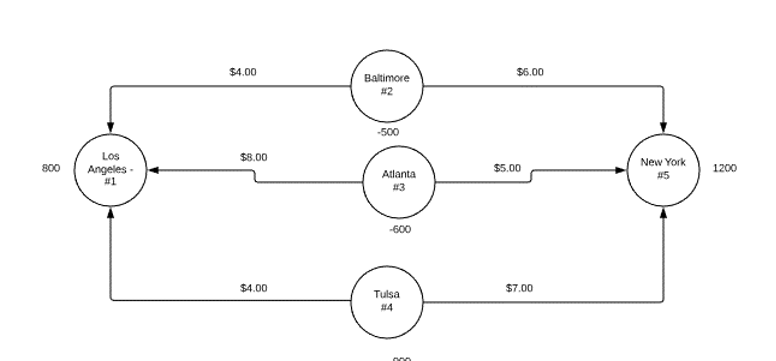
\includegraphics{Figures/Homework3/1aFig} \end{center}

\paragraph{Decision variables:}\label{decision-variables}

Let \(X_{ij}\) be the flow from node \(i\) to \(j\) where
\(i\in \{2,3,4\}\) and \(j \in \{1,5\}\)

\(X_{ij}\) are the decision variables.

\paragraph{Other variables}\label{other-variables}

Let \(C_{ij}\) be the cost variable for distribution of toys between
\(X_ij\) Let \(D_{i}\) be the supply at \(i\) and \(D_{j}\) be the
demand at \(j\). \(D_{i}\) is denoted with a negative number and the
\(D_{j}\) as positive number for modeling as a network flow problem.

\paragraph{Objective function}\label{objective-function}

\(Min\) \(Total Cost\) = \(X_{ij}C_{ij}\)

\paragraph{Constraints:}\label{constraints}

Since the supply equals the demand (\(\sum_{i}D_{i}\) \(+\)
\(\sum_{j}D_{j} = 0\)), the model will be constrained as
\(Inflow - Outflow = Supply\) \(or\) \(Demand\).

The constraints in explicit form are:

\(X_{21} + X_{31} + X_{41} - 0 = D_{1}\) where \(D_{1} = 800\)
\(X_{25} + X_{35} + X_{45} - 0 = D_{5}\) where \(D_{5} = 1200\)

\(0 - X_{21} - X_{25} = D_{2}\) Where \(D_{2} = -500\)
\(0 - X_{31} - X_{35} = D_{3}\) Where \(D_{3} = -600\)
\(0 - X_{41} - X_{45} = D_{4}\) Where \(D_{2} = -900\)

\(X_{ij} > = 0\) and \(X_{ij}\) are integers

\subsubsection{ASME Modeling}\label{asme-modeling}

Figures 1 and 2 show the model set up in ASPE

\begin{figure}
\centering
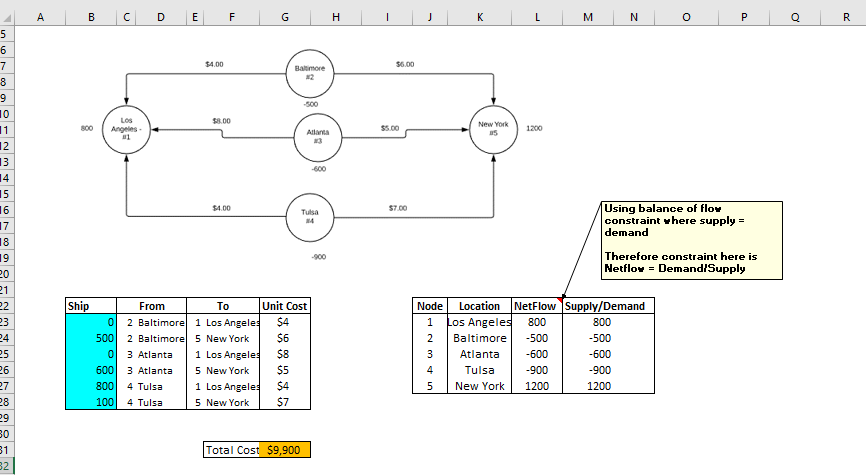
\includegraphics[height=0.50000\textwidth]{Figures/Homework3/p1a.PNG}
\caption{Problem 1 ASPE formulation}
\end{figure}

\begin{figure}
\centering
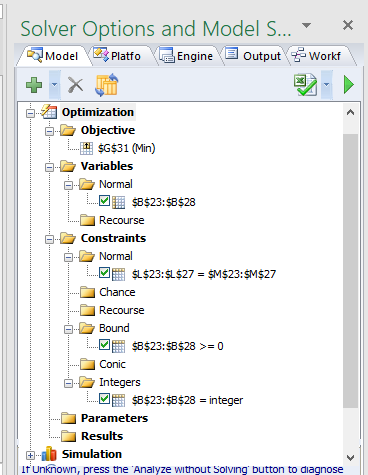
\includegraphics[height=0.50000\textwidth]{Figures/Homework3/modelp1a.PNG}
\caption{Problem 1 ASPE Model setup}
\end{figure}

\subsubsection{Scenario 1 Results}\label{scenario-1-results}

The Total cost for a plant in Baltimore was \$9900

\subsection{Scenario 2}\label{scenario-2}

\begin{figure}
\centering
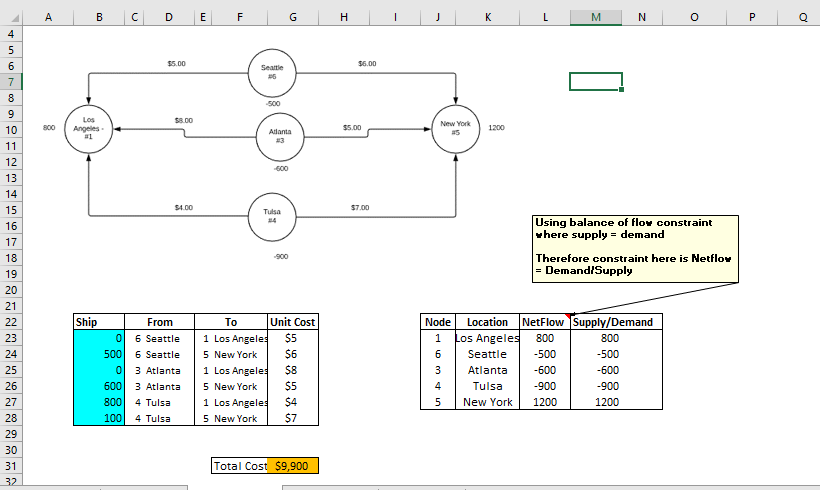
\includegraphics[height=0.50000\textwidth]{Figures/Homework3/p1b.PNG}
\caption{Problem 1 ASPE formulation}
\end{figure}


\end{document}
